\section{Interface graphique}

\label{cli}

\subsection*{Problématique}

Après avoir travaillé sur le fonctionnement général du jeu, il est intéressant de développer une nouvelle manière de visualiser une partie. On veut notamment pouvoir naviguer entre les tours, avoir un maximum d'information sur la partie. 
On s'impose également de développer cette interface en C standard.

\begin{summary}
La conception flexible du code permet d'intégrer facilement une interface graphique au jeu. Cela offre une manière plus simple de visualiser une partie.
\end{summary} 

\subsection{Stratégie}

Grâce à la structure de partie (cf \ref{game}), on a accès à l'ensemble des tours d'une partie donnée. On a donc besoin de savoir afficher un tour en entier. Pour cela on scinde l'écran en plusieurs parties.

\begin{figure}[H]
    \centering
    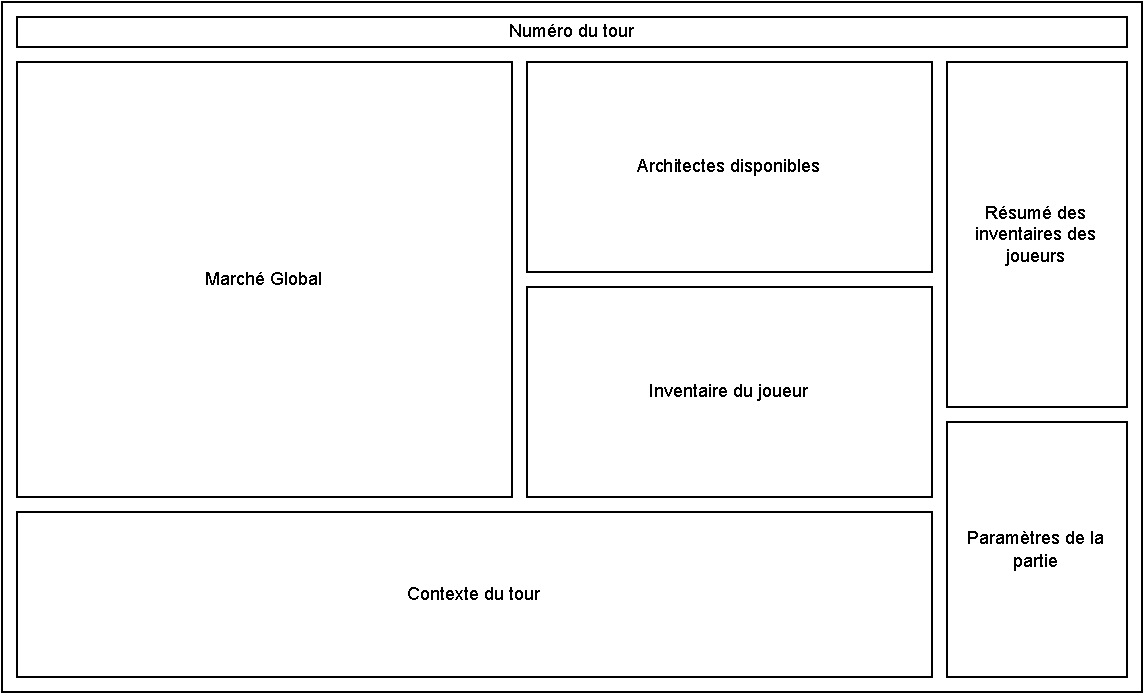
\includegraphics[width=\textwidth]{img/cli_schema.pdf}
    \caption{Schéma de l'interface}
    \label{fig:cli_schem}
\end{figure}

\subsection{Mise en oeuvre}
A l'aide de la fonction \code{print\_to\_coordinates} on est capable d'écrire aux coordonnées (x,y) le texte que l'on souhaite.

Par la suite, on doit réécrire toutes les fonctions d'affichage afin de pouvoir afficher les composants aux coordonnées souhaitées. On réutilise la même arborescence du code que pour le code principal. Un nouvel executable \code{cli} est alors créé (comme pour les tests \ref{tests} et l'évaluation de parties \ref{evaluator} ) pour jouer une partie et l'afficher.  

Pour naviguer entre les tours, on récupère l'entrée de l'utilisateur à l'aide de \code{getchar} et on décide quel tour on souhaite afficher. On peut naviguer avec les touches 'n' et 'p' ou bien les flèches.

\begin{lstlisting}[frame=single, caption={Navigation dans les tours de la partie}]
while (ch != 'q')
{
    switch (ch)
    {
        /* get the right turn to display */
    } 
    
    /* display the turn */
    cli_turn_display(turn);

    ch = getch();
}
\end{lstlisting}

\begin{summary}
Lorsque qu'on essaye d'aller au delà du dernier tour, on affiche la page des résultats avec un feu d'artifice.
\end{summary}